% -*- mode: latex; TeX-engine: xetex; LaTeX-command-style: (("" "SOURCE_DATE_EPOCH=0 %(PDF)%(latex) --shell-escape %S%(PDFout)")); TeX-master: "../dissertation.tex"; -*-

\chapter{Interaction of Single Atoms}
\label{ch:interaction-shift}

\section{Introduction}
\label{ch:interaction-shift:introduction}

The interaction between the atoms is governed by the short range molecular potential.
For low energy processes involving atoms with long de Broglie wavelengths, however,
the complex short range part of the interaction
can be ignored and the collision is approximately described by a single number,
the $s$-wave scattering length $a$.
Measuring the scattering length between the atoms allows us to probe the properties
of the molecular potential and refine predictions needed for molecule formation,
e.g. the binding energy, without direct observation of the molecular states.
Traditionally, such measurements are done either by scattering in bulk gases
or by spectroscopy in optical lattices, both of which require the preparation
of many atoms in quantum degeneracy.
The preparation of two single atoms in the motional ground state in a single tweezer,
however, allows us to cleanly perform this measurement using only two atoms
and not be affected by many-body effects that inevitably exist using the traditional approach.

In this chapter, we will discuss our measurement of the interspecies scattering lengths
between multiple Na and Cs spin states using interaction shift spectroscopy.
We will start in section~\ref{ch:interaction-shift:theory}
with a theoretical description of two interacting atoms in an optical tweezer.
The experimental techniques and the result of the measurement will be described
in section~\ref{ch:interaction-shift:spectroscopy}.
The discussion here is based on our publication in~\cite{hood_multichannel_2020}.

\section{Two Interacting Atoms in Optical Tweezer}
\label{ch:interaction-shift:theory}

The Hamiltonian for two atoms in an harmonic potential with interaction is,
\[
  H=\sum_{i=x,y,z}\paren{\frac{m_{1}\omega_{1,i}^2r_{1,i}^2}{2}+\frac{p_{1,i}^2}{2m_{1}}}+\sum_{i=x,y,z}\paren{\frac{m_{2}\omega_{2,i}^2r_{2,i}^2}{2}+\frac{p_{2,i}^2}{2m_{2}}}+V_{\mathrm{int}}\paren{\mathbf{r}_1-\mathbf{r}_2}\numberthis{eq:interaction-shift:orig-hamiltonian}
\]
where $m_j$ is the mass of the $j$-th atom,
$r_{j,i}$, $p_{j,i}$, $\omega_{j,i}$ are the coordinate, momentum and trapping frequency
for the $j$-th atom along the $i$-th axis.
$V_{\mathrm{int}}$ is the interaction potential between the two atoms which is only a function
of the relative coordinate between the atoms $\mathbf{r}_1-\mathbf{r}_2$.

Since the two atoms experience the same trapping light field,
their trapping potential has the same center and the same shape.
However, due to the difference in the polarizability between the atoms,
the trap depth can be different.
Nevertheless, in our experiment, depending on the trapping wavelength,
we have $\omega_{1,i}\approx\omega_{2,i}$ to within $10~\mathrm{\%}$ to $20~\mathrm{\%}$
and this is the regime we will mainly focus on in this section.

In order to calculate the interaction term, we can change from the coordinates for
the two individual atoms to the center of mass~(COM) and relative coordinates.
\begin{align*}
  R_i=&\ \frac{m_1r_{1,i}+m_2r_{2,i}}{m_1+m_2}&r_{\mathrm{rel},i}=&\ r_{1,i}-r_{2,i}\\
  P_i=&\ p_{1,i}+p_{2,i}&p_{\mathrm{rel},i}=&\ \frac{m_2p_{1,i}-m_1p_{2,i}}{m_1+m_2}
\end{align*}
The corresponding masses and trapping frequencies are,
\begin{align*}
  M=&\ m_1+m_2&\mu=&\ \frac{m_1m_2}{m_1+m_2}\\
  \Omega_i^2=&\ \frac{m_1\omega_{1,i}^2+m_2\omega_{2,i}^2}{m_1+m_2}&\omega_{\mathrm{rel},i}^2=&\ \frac{m_2\omega_{1,i}^2+m_1\omega_{2,i}^2}{m_1+m_2}
\end{align*}
and the Hamiltonian can be expressed as,
\begin{align*}
  \begin{split}
    H=&\sum_{i=x,y,z}\paren{\frac{M\Omega_{i}^2R_{i}^2}{2}+\frac{P_{i}^2}{2M}}+
    \left[\sum_{i=x,y,z}\paren{\frac{\mu\omega_{\mathrm{rel},i}^2r_{\mathrm{rel},i}^2}{2}+\frac{p_{\mathrm{rel},i}^2}{2\mu}}+
      V_{\mathrm{int}}\paren{\mathbf{r}_{\mathrm{rel}}}\right]\\
    &+\sum_{i=x,y,z}\mu\paren{\omega_{1,i}^2 - \omega_{2,i}^2}R_ir_{\mathrm{rel},i}
  \end{split}\numberthis{eq:interaction-shift:full-hamiltonian}
\end{align*}
The first term and the second term only rely on the COM motion and relative motion
respectively and can be solved independently. The third term mixes the COM and relative motion
and is proportional to the difference in trapping frequency.
If the trapping frequencies are the same for the two atoms, the third term is $0$ and
the solution is fully separable.
As mentioned above, since the trapping frequencies for the two atoms are similar,
we will assume the mixing term is small and treat it as a small correction in the calculation.

The interaction potential $V_{\mathrm{int}}$ gives rise to
the molecular bound states and its exact form will be discussed in chapter~\ref{ch:pa},
\ref{ch:raman-spectroscopy} and \ref{ch:raman-transfer}.
However, since the range of the potential is much smaller than
the size of the atomic wavefunction, we can ignore the short range details of the potential
and treat it as a contact interaction characterized only by
the scattering length $a$~\cite{busch_two_1998},
\[
  V_{\mathrm{int}}\paren{\mathbf{r}}=\frac{2\pi\hbar^2a}{\mu}\delta_{\mathrm{reg}}\paren{\mathbf{r}}
\]
where $\mu = m_1m_2/\paren{m_1+m_2}$ is the reduced mass and
$\delta_{\mathrm{reg}}\paren{\mathbf{r}}\equiv\delta^{(3)}\paren{\mathbf{r}}\paren{\partial/\partial r}r$
is the regularized delta-function. This pseudo-potential is valid
when the van der Waals length~$\beta_6 = (2\mu C_6 / \hbar^2)^{1/4}$
is much smaller than the relative harmonic oscillator lengths~$\beta_{\mathrm{rel},i}$~\cite{
  bolda_effective-scattering-length_2002,blume_fermi_2002}.
In our experiment, these are $\beta_6 \approx 6~\mathrm{nm}$,
$\beta_{\mathrm{rel},x} \approx \beta_{\mathrm{rel},y}\approx 66~\mathrm{nm}$ for the radial axes,
and  $\beta_{\mathrm{rel},z} \approx 158~\mathrm{nm}$ for the axial axis.

\subsection{Perturbative Calculation}
\label{ch:interaction-shift:theory:perturb}

For weak interaction, i.e. a small scattering length $a$, the effect of the interaction
on the energies can be calculated perturbatively.
The result from this calculation is useful for checking the validity of the full calculation,
as well as providing an intuitive understanding of the shift and its dependence
on different parameters.

For simplicity, we will assume all the trapping frequencies are the same,
i.e. $\omega_{1,i}=\omega_{2,i}=\omega_{\mathrm{rel},i}=\Omega_i=\omega_i$,
so that we only need to consider the relative motion,
\[
  H_{\mathrm{rel}}=\sum_{i=x,y,z}\paren{\frac{\mu\omega_{i}^2r_{\mathrm{rel},i}^2}{2}+\frac{p_{\mathrm{rel},i}^2}{2\mu}}+
  V_{\mathrm{int}}\paren{\mathbf{r}_{\mathrm{rel}}}
\]
When treating the interaction as perturbation, the base solution is the harmonic oscillator
states for the relative motion $|n_{\mathrm{rel},x},n_{\mathrm{rel},y},n_{\mathrm{rel},z}\rangle$.
The energy level perturbation is then,
\begin{align*}
  \Delta_{n_{\mathrm{rel},x},n_{\mathrm{rel},y},n_{\mathrm{rel},z}}=&\langle n_{\mathrm{rel},x},n_{\mathrm{rel},y},n_{\mathrm{rel},z}|V_{\mathrm{int}}\paren{\mathbf{r}_{\mathrm{rel}}}|n_{\mathrm{rel},x},n_{\mathrm{rel},y},n_{\mathrm{rel},z}\rangle\\
  =&\frac{2\pi\hbar^2a}{\mu}\langle n_{\mathrm{rel},x},n_{\mathrm{rel},y},n_{\mathrm{rel},z}|\delta_{reg}\paren{\mathbf{r}_{\mathrm{rel}}}|n_{\mathrm{rel},x},n_{\mathrm{rel},y},n_{\mathrm{rel},z}\rangle\\
  =&\frac{2\pi\hbar^2a}{\mu}\abs{\psi_{n_{\mathrm{rel},x},n_{\mathrm{rel},y},n_{\mathrm{rel},z}}(0)}^2\numberthis{eq:interaction-shift-perturb-shift}
\end{align*}
where $\abs{\psi_{n_{\mathrm{rel},x},n_{\mathrm{rel},y},n_{\mathrm{rel},z}}(0)}^2$ is the probability density
for zero distance between the atoms.

For the motional ground state, the shift is,
\begin{align*}
  \Delta_{0,0,0}=&a\frac{2\hbar^2}{\mu\sqrt{\pi}}\prod_{i=x,y,z}\frac{1}{\beta_{\mathrm{rel},i}}
\end{align*}
where $\beta_{\mathrm{rel},i}\equiv\sqrt{\hbar/\mu\omega_{\mathrm{rel},i}}$ is the relative motion
oscillator length along the $i$-th axis.
The shift is proportional to the strength of the interaction $a$,
and is also bigger for stronger confinement where the wavefunction density is higher.

We can see from Eq.~\ref{eq:interaction-shift-perturb-shift} that the shift is only
non-zero when all of $n_{\mathrm{rel},i}$'s are even.
The shift is also smaller for higher motional excited states
with lower wavefunction density at $\mathbf{r}_{\mathrm{rel}}=0$.
This means that the shift will only be observable if the atom is cooled to close to
the motional ground state and will be small or zero for other states.

\subsection{Non-perturbative Calculation}
\label{ch:interaction-shift:theory:non-perturb}

The first order perturbative result breaks down for large $a$ when the energy shift
approaches the motional energy scale $\omega_{\mathrm{rel},i}$.
Moreover, due to the divergent nature of the delta-function in the contact interaction potential,
higher order perturbative calculations do not converge.
It is therefore necessary to use a non-perturbative solution of the interacting atoms
in order to interpret measurements of the shift for strong interaction.
To do this, we first ignore the last term in
the Hamiltonian~\ref{eq:interaction-shift:full-hamiltonian} so that it is fully separable
into COM and relative motion.
This term, along with a few other corrections,
will be added later numerically to obtain the full solution.

For the relative Hamiltonian, we use the analytical cylindrical solutions
from Ref.~\cite{idziaszek_analytical_2006}.
These solutions require the potential to be cylindrically symmetric and
that the ratio between the radial trapping frequency
and the axial trapping frequency $\eta\equiv\omega_{\mathrm{radial}}/\omega_z$
to be an integer.
We therefore define $\eta = 6$, which is close to the actual values of $5.6$
and ignores the $7~\mathrm{\%}$ difference between the two radial trapping frequencies
in order to use these solutions.
These differences from the real Hamiltonian will be included later as a correction~\cite{
  bertelsen_association_2007,deuretzbacher_heteronuclear_2008}.

Moreover, Ref.~\cite{idziaszek_analytical_2006} does not provide the wavefunctions
for the full solution, but only include the ones for the interacting states.
In order to use the solution, we must expand it to include the non-interacting states as well.
We have identified these states from the perturbative calculation
in section~\ref{ch:interaction-shift:theory:perturb}
which are the ones witch at least one odd $n_{\mathrm{rel},i}$.
In order to match the analytical solution,
we can transform to the cylindrical harmonic oscillator basis.
The eigenenergies becomes
\begin{align*}
  \frac{E_{n,l,m_z}}{\hbar\omega_z}=&\paren{2 n + |l| + 1}\eta + \paren{m_z + 1/2}
                                      \numberthis{eq:interaction-shift:cylind-E}
\end{align*}
where $n$ is the principal quantum number for the radial part,
$l$ is the angular momentum quantum numbers for the radial part,
and $m_z$ is quantum number for the axial 1D harmonic oscillator.
The condition for non-interacting states becomes $l\ne0$ or odd $m_z$.
However, when $\eta$ is an integer, as is required by the solution of the interacting states,
there is a subspace of cylindrical harmonic oscillator states with $l=0$
and even $m_z$ that are degenerate from Eq.~\ref{eq:interaction-shift:cylind-E}.
This accidental degeneracy reduces the number of interacting states such that
within each degenerate subspace with $N_{\mathrm{deg}}$ states,
there is only one interacting state and the rest $N_{\mathrm{deg}}-1$ states are non-interacting.
We can express a non-interacting state $\psi_{\mathrm{non-int}}$ within this subspace
as a superposition of the cylindrical harmonic oscillator states
$\psi_{\mathrm{non-int}}=\sum_ic_i\psi_i$,
where the sum is over all the spaces in the degenerate subspace.
The state must satisfy the condition $V_{\mathrm{int}}\psi_{\mathrm{non-int}} = 0$ or
$\psi_{\mathrm{non-int}}\paren{\mathbf{r}_{\mathrm{rel}}=0}=0$.
We find these amplitudes $c_i$ using a Gram-Schmidt procedure, based on the requirement
$\sum_{i=1}^{N_{\mathrm{deg}}} c_i \psi_i\paren{\mathbf{r}_{\mathrm{rel}}=0} = 0$.
The procedure identifies $N_{\mathrm{deg}}-1$ non-interacting states within the subspace
which is combined with the interacting state from Ref.~\cite{idziaszek_analytical_2006}
to form the full solution.

For the interacting states,
the energies are given by the transcendental equations~\cite{idziaszek_analytical_2006}
\begin{align*}
  \mathcal{F}\paren{-\frac{\paren{E-E_0}}{2}, \eta}=&-\frac{\sqrt{2\pi}}{a}
\end{align*}
where $\mathcal{F}\paren{x, \eta}$ is given by
\begin{align*}
  \mathcal{F}\paren{x, \eta}=
  &\frac{\sqrt{\pi} \Gamma(x)}{\Gamma(x+\frac{1}{2})}
    \sum_{m=1}^{n-1} F\paren{1,x;x+\frac{1}{2} ; e^{\ui(2\pi m/ \eta)}}
    -\frac{2 \sqrt{\pi} \Gamma(x)}{\Gamma(x-\frac{1}{2})}
\end{align*}
Here $F(a,b;c,x)$ denotes the hypergeometric function
and $\Gamma(x)$ is the Euler gamma function.
The energy $E$ and $E_0$ are in units of the axial trapping frequency $\omega_z$,
and so the ground-state energy $E_0 = \eta + 1/2$.

The COM Hamiltonian is a cylindrical harmonic oscillator and the energy is given by
Eq.~\ref{eq:interaction-shift:cylind-E}.

\begin{figure}
  \centering
  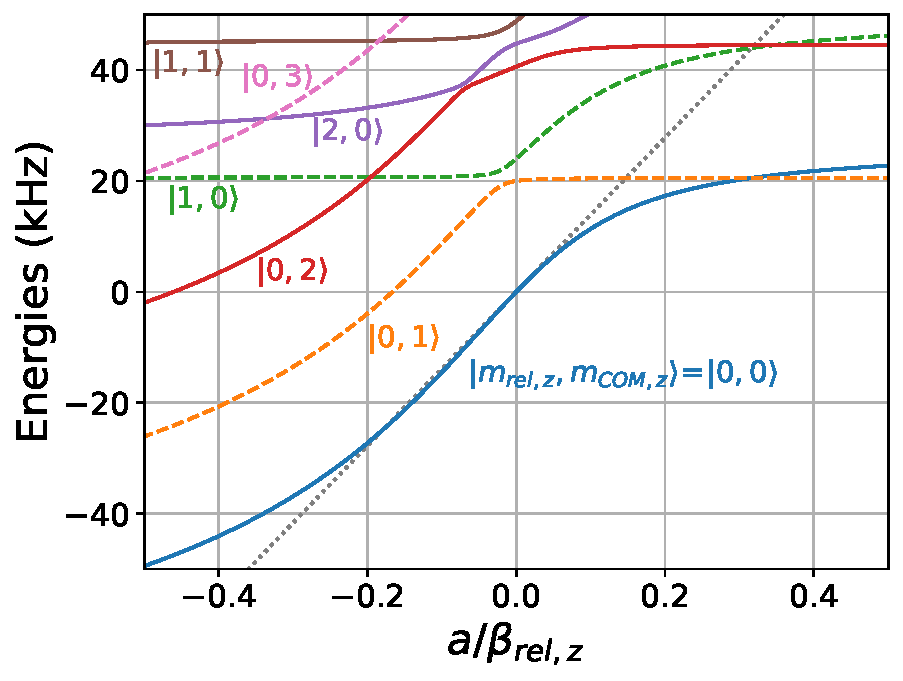
\includegraphics[width=0.7\textwidth]{figures/interaction_shift_energies.pdf}
  \caption[Result of interaction shift calculation.]{
    Energy levels as a function of scattering length
    (in unit of the axial relative motion oscillator length
    $\beta_{\mathrm{rel},z}$) from the non-perturbative calculation.
    The dashed straight light is the result from first order perturbation
    for the motional ground state which shows good agreement with the exact calculation
    at small scattering length.
    Only states that are in the radial motional (both relative and COM) ground state
    are shown because of the high radial motional energy scale~($100~\mathrm{kHz}$).
    The states are labeled with their relative and COM axial motional quantum numbers
    $m_{\mathrm{rel},z}$ and $m_{\mathrm{COM},z}$.
    Due to the relative and COM motion mixing term and the resulting avoided crossings
    in the energy levels, these are not the true quantum numbers
    and are not constants along the same line.
    The numbers shown in the plot are for the state at large negative scattering length.
    States with even total parity, i.e. $m_{\mathrm{rel},z} + m_{\mathrm{COM},z}$, are plotted in solid lines
    whereas ones with odd total parity are plotted in dashed lines.
    Since the Hamiltonian conserves total parity,
    there is no coupling between the two sets of states
    which results in the level crossing shown in the plot.
    \label{fig:interaction-shift:energies}}
\end{figure}

Now that we have the solution in the separable and cylindrical case,
the next step is to include the correction terms from the effects that were ignored above.
These include the COM and relative motion mixing term
from the Hamiltonian~\ref{eq:interaction-shift:full-hamiltonian},
the asymmetry of the two radial axis, and the effect of non-integer $\eta$.
The total matrix is diagonalized in the combined COM and relative cylindrical bases.
Compared to treating the interaction term in Eq.~\ref{eq:interaction-shift:orig-hamiltonian}
as a perturbation, the correction terms included here all have the form of
harmonic potentials and therefore have much better convergence behavior.
We include all states with energies up to $20 \omega_{\mathrm{rel},z}$ in the calculation.
The matrix elements are calculated numerically using the cylindrical wavefunctions,
which for completeness are given here:
\begin{align*}
  \Psi_{n,l,m_z}\paren{\rho,\theta,z}=
  &\Psi^{\mathrm{radial}}_{n,l}\paren{\rho, \theta}\Psi^{\mathrm{axial}}_{m_z}\paren{z}
\end{align*}
with the normalized radial harmonic oscillator wavefunction,
\begin{align*}
  \Psi^{\mathrm{radial}}_{n,l}\paren{\rho, \theta}=
  &\sqrt{\frac{2n!}{a_\perp^2 (n+|l|)!}} e^{-r^2/(2 a_\perp^2)} \paren{\frac{r}{a_\perp}}^{|l|}
    L_n^{|l|}\paren{\frac{r^2}{a_\perp^2}} \frac{ e^{i l \theta}}{\sqrt{2 \pi}}
\end{align*}
and the normalized 1D harmonic wavefunction,
\begin{align*}
  \Psi^{\mathrm{axial}}_{m_z}(z)=&\frac{1}{\sqrt{2^{m_z} m_z!}} \frac{1}{\sqrt{a_z}(\pi)^{1/4}}
                                   e^{-z^2/(2 a_z)} H_{m_z}(z/a_z)
\end{align*}
Here the radial and axial oscillator lengths are defined as
$a_\perp = \sqrt{\hbar/(\mu \omega_\perp)}$ and $a_z = \sqrt{\hbar/ (\mu \omega_z)}$.
$H_{m_z}$ are the Hermite-Gaussian functions,
and $L^{|l|}_n$ are the generalized Laguerre polynomials.

The eigenenergies of the matrix are calculated as a function of the scattering length.
The results for the lowest energy ones are shown in Fig.~\ref{fig:interaction-shift:energies}.

\section{Interaction Shift Spectroscopy}
\label{ch:interaction-shift:spectroscopy}

\subsection{Experiment Sequence}
\label{ch:interaction-shift:spectroscopy:sequence}
The absolute energies shown in Fig.~\ref{fig:interaction-shift:energies} have an arbitrary global
offset and are therefore not directly measurable.
Instead, the measurable quantities are the energy differences between different states,
which can be done either by changing the scattering length,
i.e. moving along the x axis in Fig.~\ref{fig:interaction-shift:energies},
or by changing the motional state of the atoms, i.e. moving along the y axis.

\begin{figure}
  \centering
  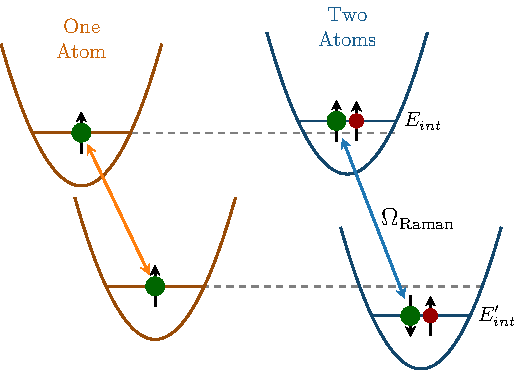
\includegraphics[width=0.7\textwidth]{figures/interaction_shift_measure.pdf}
  \caption[Schematics of interaction shift spectroscopy.]{
    Schematics of interaction shift spectroscopy using Raman transitions.
    Left: Raman resonance for atomic spin flip with only one atom in the tweezer.
    Right: The energy shifts by a spin state dependent amount with the present of
    the second~(red) atom. This causes a shift in the spin flip resonance frequency
    for the first~(green) atom compared to the one atom case.
    The shift corresponds to the difference in the interaction shift between the
    two spin states.
    \label{fig:interaction-shift:measure}}
\end{figure}

In our experiment, we measure the interaction shifts by flipping the spin state of
one but not the other atom using Raman transitions.
Since the scattering length depends on the spin state,
the interaction shift may be different between the initial and final spin states.
We measure this difference by comparing the resonance frequency in the absence of
the other atom~(Fig.~\ref{fig:interaction-shift:measure}).
The spin flip is done in the same $8.8~\mathrm{G}$ we use for
Raman sideband cooling~(section~\ref{ch:rsc:setup}).
We drive the transition using two Raman beams that are co-propagating
which imprints no phase gradient on
the atomic wavefunction~(section~\ref{ch:rsc:basic-theory:raman}).
This reduces the number of observable resonances and provides a cleaner spectrum since,
\begin{enumerate}
\item Parity is conserved during the transition.\\
  Starting from the motional ground state, this means that all dashed lines in
  Fig.~\ref{fig:interaction-shift:energies} are uncoupled.
\item Coupling to different motional states are surppressed.\\
  In particular, this reduces the coupling to COM motional excitation
  in the strong interaction limit.
  Note that since the interaction between the atoms modifies the wavefunction,
  there is still non zero overlap between different motional states
  especially for the relative motion.
\end{enumerate}

\subsection{Results}
\label{ch:interaction-shift:spectroscopy:results}

\begin{figure}
  \centering
  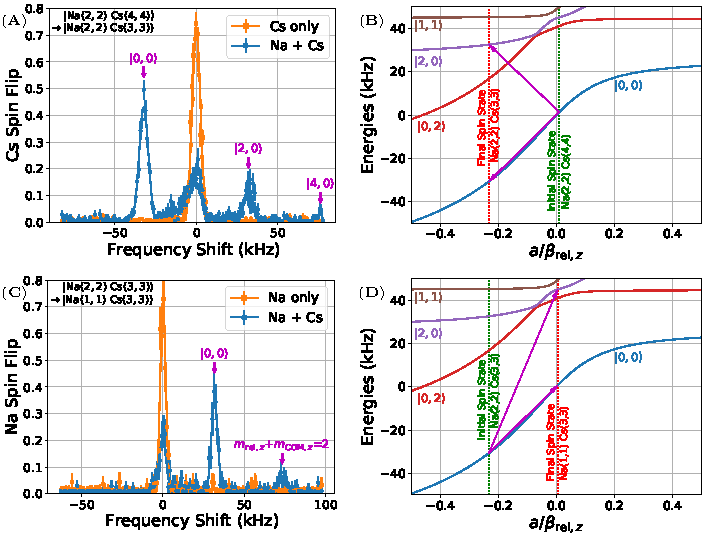
\includegraphics[width=\textwidth]{figures/interaction_shift_results.pdf}
  \caption[Interaction shift measurement results.]{
    Interaction shift measurement for
    (A) $|\mathrm{Na(2, 2),Cs(4, 4)}\rangle\rightarrow|\mathrm{Na(2, 2),Cs(3, 3)}\rangle$
    and (C) $|\mathrm{Na(2, 2),Cs(3, 3)}\rangle\rightarrow|\mathrm{Na(1, 1),Cs(3, 3)}\rangle$
    with the corresponding transition shown on the energy map from theoretical calculation
    in (B) and (D) respectively.
    The orange line shows the bare resonance with only one atom in the trap
    and the blue line shows the spectrum including interaction shift.
    A resonance appearing at positive frequency shift corresponds to the final state
    having a more positive energy (more repulsive interaction or higher motional energy).
    More than one shifted peaks can be observed due to the motional state mixing caused
    by the interaction. The corresponding motional state is marked as
    $|m_{\mathrm{rel},z},m_{\mathrm{COM},z}\rangle$ on the resonance.
    For the $|\mathrm{Na(2, 2),Cs(3, 3)}\rangle\rightarrow|\mathrm{Na(1, 1),Cs(3, 3)}\rangle$
    transition (C and D), the states with two quanta of total axial excitation are unresolved.
    Since the Raman transition preserves parity, only states with even parity are shown
    in (B) and (D).
    \label{fig:interaction-shift:results}}
\end{figure}

The spectrum for the $|\mathrm{Na(2, 2),Cs(4, 4)}\rangle$ to $|\mathrm{Na(2, 2),Cs(3, 3)}\rangle$
transition is shown in Fig.~\ref{fig:interaction-shift:results}A.
The orange line shows the bare $|\Cs(4, 4)\rangle$ to $|\Cs(3, 3)\rangle$ resonance without
the presence of the Na atom whereas the blue line shows the resonances
including the interaction with the Na atom.
The largest peak on the left is the shifted ground motional state
$|m_{\mathrm{rel},z},m_{\mathrm{COM},z}\rangle = |0,0\rangle$ and the smaller peak on the right
corresponds to the $|2,0\rangle$ state~(Fig.~\ref{fig:interaction-shift:results}B).
A even smaller resonance for $|4,0\rangle$ is also visible further right
(not shown in Fig.~\ref{fig:interaction-shift:results}B).
The $|0,0\rangle$ resonance gives the difference of the interaction shifts
of the initial and final spin states,
$E(\mathrm{Na(2, 2),Cs(3, 3)}) - E(\mathrm{Na(2, 2),Cs(4, 4)})=-32.1(2) \mathrm{kHz}$.
The peak near zero frequency corresponds to the initial Na and Cs population that is not prepared
in the motional ground state or an interacting state.
The fitted height $0.46$ of the $|0,0\rangle$ peak serves as a lower bound for
the relative motional ground-state population.
Similarly, Fig.~\ref{fig:interaction-shift:results}C shows the result for
the $|\mathrm{Na(2, 2),Cs(3, 3)}\rangle$ to $|\mathrm{Na(1, 1),Cs(3, 3)}\rangle$
measured by driving a Na Raman transition.
Two interaction shifted resonances were observed which corresponds to
the motional ground state and unresolved states with two total
Na and Cs motional excitation~(Fig.~\ref{fig:interaction-shift:results}D).

\begin{table}
  \centering
  \caption[Interaction shift and scattering lengths.]{
    Interaction shift and scattering lengths for different spin states.
    The number for the $|\mathrm{Na(2, 2),Cs(4, 4)}\rangle$ is computed from
    the binding energy of the molecular state whereas the other numbers are
    measured by the interaction spectroscopy.
    \label{table:interaction-shift:results}}
  \begin{tabular}{|c|c|c|}
    \hline
    Spin state&Interaction Shift (kHz)&Scattering Length\\\hline
    $|\mathrm{Na(2, 2),Cs(4, 4)}\rangle$&$1.40$&$30.4a_0$\\\hline
    $|\mathrm{Na(2, 2),Cs(3, 3)}\rangle$&$-30.7$&$-693.8a_0$\\\hline
    $|\mathrm{Na(1, 1),Cs(3, 3)}\rangle$&$0.62$&$13.7a_0$\\\hline
  \end{tabular}
\end{table}

Since the measurement only gives the energy difference
between spin state combinations with different scattering lengths,
we determine an absolute interaction shift of the $|\mathrm{Na(2, 2),Cs(4, 4)}\rangle$
using the binding energy of
the least bound state $v''=-1$~(section~\ref{ch:raman-spectroscopy:states:n0}).
The absence of spin mixing for this state allows its binding energy to be related
to the scattering length directly through
single-channel quantum defect theory~(QDT)~\cite{
  gao_quantum-defect_1998,gao_angular-momentum-insensitive_2001,gao_general_2008}
but extended to two-scale by including the $-C_8/r^8$ potential.
For the van der Waals coefficients, we use $C_6=3227~\mathrm{a.u.}$ and
$C_8=3.681\times10^5~\mathrm{a.u.}$ from
Refs.~\cite{docenko_coupling_2006,mcguyer_high-precision_2015,porsev_accurate_2003}.
From here, we can use the result of the calculation above to obtain all the
absolute interaction shifts and scattering lengths,
summarized in table~\ref{table:interaction-shift:results}.

\section{Summary and Outlook}
\label{ch:interaction-shift:summary}
Optical tweezers provide a clean platform to study the interaction between exactly two atoms.
Here, we started our exploration of the interaction by measuring the most important quantity
for $s$-wave scattering process at ultracold temperature, the scattering length $a$.
The results from these measurements can be used
to refine the theoretical model of the NaCs molecule,
including predictions of the molecule binding energy
and Feshbach resonances~\cite{hood_multichannel_2020}.
More properties of the interaction will be studied in the following chapters.

Additionally, the combination of the tight confinement from the optical tweezer
and the interaction between the atoms also gives us further control
of the motional states of the atom.
As we have seen in this chapter, the degeneracy of carrier Raman transition
for different motional states is lifted by the interaction.
As a result, driving on the interaction shifted resonance
allows us to prepare a system that is completely in the ground state of the relative motion.
This will be used when we coherently create the molecules~(chapter~\ref{ch:raman-transfer})
to lower the requirement for the cooling and reduce the background caused by hot atoms.
